\section{Zadanie 2 (Hubert Jastrzębski)}

Poruszasz się między domem a biurem. Pewnego razu kupiłeś cztery parasole, które położyłeś w domu przy wejściu. Przyjmijmy następnie, że każdego dnia (zaczynając od Dnia 0) wychodzisz rano z domu do biura i po południu wychodzisz z biura do domu. Przed każdym takim wyjściem: jeśli w danym momencie pada deszcz i jeśli masz jeden z parasoli w swojej lokalizacji, to bierzesz parasol, chronisz się przed deszczem i odkładasz parasol w docelowej lokalizacji.

Załóżmy, że w każdym momencie prawdopodobieństwo tego, że pada wynosi $p$. Dla każdego $n \in \mathbb{N}$, niech $X_{2n}$ będzie zmienną losową określającą liczbę parasoli w domu w Dniu $n$-tym rano przed Twoim wyjściem i niech $X_{2n+1}$ będzie zmienną losową określającą liczbę parasoli w biurze w Dniu $n$-tym w czasie Twojej pracy.

\begin{enumerate}
    \item Czy $(X_n)_{n \in \mathbb{N}}$ jest łańcuchem Markowa?
    \item Jeśli odpowiedział-aś/-eś na (i) tak, to czy ten łańcuch ma rozkład stacjonarny? Jeśli tak, to oblicz ten rozkład.
    \item Dla $n \in \mathbb{N}$, niech $A_n$ będzie zdarzeniem, że $n$-tego dnia zmokł-aś/-eś: to jest wychodząc z domu lub później wychodząc z pracy padał deszcz, a Ty nie miał-aś/-eś parasola. Oblicz $\lim_{n \to \infty} P(A_n)$.
    \item Jeśli mieszkasz w Szkocji, gdzie $p = 0.6$, ile potrzebujesz kupić parasoli na starcie, aby $\lim_{n \to \infty} P(A_n) < 0.1$?
\end{enumerate}

\subsection*{Rozwiązanie}

\begin{center}
  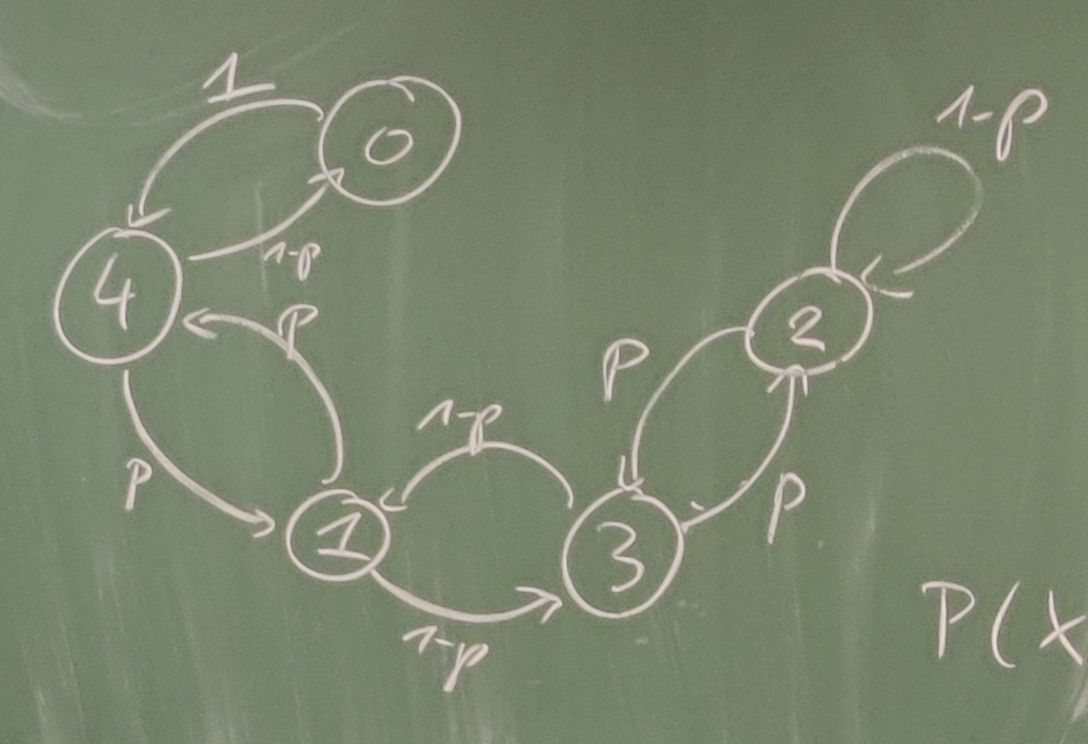
\includegraphics[width=0.7\textwidth]{tasks/02_markov.jpg} 
\end{center}

\textbf{Podpunkt 1.}
Jak widać, jest to łańcuch Markowa. Koniec.

A trochę dokładniejsze wytłumaczenie: 

Każdy z tych wierzchołków $(0), (1), (2), (3), (4)$ to liczba parasoli, które są w naszej lokalizacji. 
Czyli zaczynamy od stanu $(4)$ i jeśli nie pada deszcz, to nie bierzemy parasola i idziemy do biura w którym jest $4 - 4 = 0$ parasoli (stan $(0)$).
Jeśli natomiast pada deszcz, to bierzemy parasol i idziemy do biura w którym jest $4 - 4 + 1 = 1$ parasol (stan $(1)$).
Analogicznie dla innych stanów; jeśli jesteśmy w $(k)$ i pada, to bierzemy parasol i zwiększamy liczbę w tej drugiej lokazliacji (gdzie jest $4 - k + 1$ parasoli), a jeśli nie pada to nie bierzemy i jest $4 - k$ parasoli.

Dany stan zależy tylko od poprzedniego, bo nie obchodzi nas, czy jesteśmy w domu, czy w biurze, tylko to ile mamy koło siebie parasoli.

\textbf{Podpunkt 2.}
Ma rozkład stacjonarny. Możemy to policzyć na dwa sposoby:

\textbf{Sposób 1.}

Aby znaleźć rozkład stacjonarny, musimy rozwiązać równanie $\pi P = \pi$, gdzie $P$ to macierz przejścia, a $\pi = (\pi_0, \pi_1, \pi_2, \pi_3, \pi_4)$ to wektor rozkładu stacjonarnego.

Macierz przejścia $P$ jest następująca:
\[
P = \begin{pmatrix}
 & \mathbf{0} & \mathbf{1} & \mathbf{2} & \mathbf{3} & \mathbf{4} \\
\mathbf{0} & 0 & 0 & 0 & 0 & 1 \\
\mathbf{1} & 0 & 0 & 0 & 1-p & p \\
\mathbf{2} & 0 & 0 & 1-p & p & 0 \\
\mathbf{3} & 0 & 1-p & p & 0 & 0 \\
\mathbf{4} & 1-p & p & 0 & 0 & 0
\end{pmatrix}
\]

Tak więc mnożymy wektor $\pi$ przez macierz $P$ i przyrównujemy do $\pi$:
\[
\begin{cases}
\pi_4(1-p) = \pi_0 \quad & (1) \\
\pi_3(1-p) + \pi_4 p = \pi_1 \quad & (2) \\
\pi_2(1-p) + \pi_3 p = \pi_2 \quad & (3) \\
\pi_1(1-p) + \pi_2 p = \pi_3 \quad & (4) \\
\pi_0 + \pi_1 p = \pi_4 \quad & (5) \\
\sum_{k=0}^{4} \pi_k = 1 \quad & (6)
\end{cases}
\]

Z równania (3) otrzymujemy $\pi_2(1 - (1-p)) = \pi_3 p \implies \pi_2 = \pi_3$.
Podstawiając to do (4) mamy $\pi_1(1-p) + \pi_2 p = \pi_2 \implies \pi_1 = \pi_2$.
Następnie z (2), wiedząc że $\pi_3 = \pi_1$, mamy $\pi_1(1-p) + \pi_4 p = \pi_1 \implies \pi_4 = \pi_1$.

Mamy więc równość stanów: $\pi_1 = \pi_2 = \pi_3 = \pi_4$.
Z równania (1) wyznaczamy $\pi_0$: $\pi_0 = (1 - p)\pi_4$.

Podstawiamy do warunku sumowania (6):
\[
(1-p)\pi_4 + 4\pi_4 = 1 \implies \pi_4(1 - p + 4) = 1 \implies \pi_4 = \frac{1}{5 - p}
\]

Ostatecznie:
\[
\pi_0 = \frac{1 - p}{5 - p}, \quad \pi_1 = \pi_2 = \pi_3 = \pi_4 = \frac{1}{5 - p}
\]

\textbf{Sposób 2.} (ten nieszczęsny)

Skorzystamy z \href{https://en.wikipedia.org/wiki/Balance\_equation}{Global balance equation}.

Dla dowolnego podzbioru stanów $X \subset S$:

$$\underbrace{\sum_{x \in X} \left( \pi_x \sum_{y \notin X} p_{xy}\right)}_{\text{Wypływ z } X} = \underbrace{\sum_{y \notin X} \left( \pi_y \sum_{x \in X} p_{yx}\right)}_{\text{Wpływ do } X}$$

$$ \iff \pi \text{ jest rozkładem stacjonarnym}$$ 

Zauważmy jednak, że nie musimy sprawdzać wszystkich podzbiorów \(S\).
Jeśli sprawdzimy tylko singletony, to wystarczy, ponieważ dla dowolnego podzbioru \(X\) możemy rozbić sumę na sumy po singletonach.

Jeszcze tylko przypomnijmy, że \(p_{xy}\) to prawdopodobieństwo przejścia ze stanu \(x\) do stanu \(y\)
(nie pamiętam, czy na wykładzie było tak, czy na odwrót?).

Sprawdzamy więc dla każdego stanu:
Sprawdzamy więc bilans przepływu (wychodzące poza stan = wchodzące spoza stanu) dla każdego stanu:
\begin{enumerate}
    \item Dla $X = \{0\}$: $\pi_0 \cdot (1) = \pi_4 \cdot (1 - p)$
    \item Dla $X = \{1\}$: $\pi_1 \cdot (1) = \pi_3 \cdot (1 - p) + \pi_4 \cdot p$
    \item Dla $X = \{2\}$: $\pi_2 \cdot p = \pi_3 \cdot p$ \quad (nie liczymy po żadnej stronie 2 $\rightarrow$ 2 !)
    \item Dla $X = \{3\}$: $\pi_3 \cdot (1) = \pi_1 \cdot (1 - p) + \pi_2 \cdot p$
    \item Dla $X = \{4\}$: $\pi_4 \cdot (1) = \pi_0 \cdot (1) + \pi_1 \cdot p$
\end{enumerate}

Podobnie jak w Sposobie 1, rozwiązując te równania wraz z warunkiem sumowania, otrzymujemy ten sam rozkład stacjonarny.

\textbf{Podpunkt 3.}
Zdarzenie $A_n$ zachodzi, gdy pada deszcz i nie mamy parasola w domu lub w biurze.

Trzeba pamiętać, że dzień składa się z dwóch wyjść: z domu do biura i z biura do domu!

Czyli $A_n = \{(X_{2n} = 0 \land \text{ pada }) \lor (X_{2n+1} = 0 \land \text{ pada })\}$

Zauważmy też, że te zdarzenia są rozłączne. 
Jest tak, ponieważ liczba parasoli w domu i w biurze sumuje się do 4, więc jeśli zmoknę rano, to nie zmoknę po południu nawet jak będzie padać deszcz.
Zatem:  
\begin{align*}
    P(A_n) &= P(X_{2n} = 0 \land \text{ pada}) + P(X_{2n+1} = 0 \land \text{ pada}) \\
    &= p \cdot \pi_0 + p \cdot \pi_0 = 2p \pi_0 \text{ , dla n } \to \infty
\end{align*}

Czemu $p \cdot \pi_0$? Bo liczymy granicę, a po długim czasie zawsze rozkład zbliża się do rozkładu stacjonarnego.
Natomiast w stanie stacjonarnym $P(X_n = k) = \pi_k$ dla każdego $n$.


\[
\lim_{n \to \infty} P(A_n) = 2 \cdot (p \cdot \pi_0) = \frac{2p(1 - p)}{5 - p}
\]


\textbf{Podpunkt 4.}

Uogólniamy wzór na $\pi$ dla $N$ parasoli. 

Zauważmy, że do stanu \((0)\) możemy przejść tylko ze stanu \((N)\) gdy nie pada, tak więc \[\pi_0 = (1-p)\pi_N\]

Możemy udowodnić też, że dla takiego \(\pi_0\) oraz \(\pi_1 = \pi_2 = \ldots = \pi_N = x\), $\pi$ jest rozkładem stacjonarnym. Wystarczy skorzystać z global balance equation dla singletonów, podobnie jak w Podpunkcie 2:

Dla każdego \(k \in \{1, 2, \ldots, N-1\}\)
rozważamy stan \(X = \{k\}\): 
\[\pi_k = \pi_{N - k} \cdot (1 - p) + \pi _{N - k + 1} \cdot p\]
\[x = x \cdot (1 - p) + x \cdot p\]
\[x = x \text{ co jest prawdziwe}\]
Tak więc dla każdego \(k\) od 1 do \(N-1\) równanie jest spełnione.
Dla \(k = 0\) mamy już udowodnione, a dla \(k = N\) rozważamy stan \(X = \{N\}\):
\[\pi_N = \pi_0 + \pi_1 \cdot p\]
\[x = (1 - p)x + x \cdot p\]
\[x = x \text{ co jest prawdziwe}\]

Tak więc jest to rzeczywiście poprawny rozkład stacjonarny. 
Wiemy, że sumuje się do 1, więc możemy wyznaczyć \(x\):
\[(1 - p)x + N \cdot x = 1\]
\[x = \frac{1}{N + 1 - p}\]

Dzięki temu możemy policzyć ogólny wzór na prawdopodobieństwo zmoknięcia w ciągu dnia:
\[
P(A_n) = \frac{2p(1 - p)}{N + 1 - p}
\]

Dla Szkocji ($p = 0.6$) szukamy $N$, aby wynik był $< 0.1$:

\[
\frac{2 \cdot 0.6 \cdot 0.4}{N + 0.4} < 0.1
\]
\[
\frac{0.48}{N + 0.4} < 0.1 \quad \Big| \cdot 10(N+0.4)
\]
\[
4.8 < N + 0.4
\]
\[
N > 4.4
\]

Najmniejszą liczbą naturalną jest $N = 5$.

\subsection*{Odpowiedź}
\[
\boxed{\begin{aligned}
\text{(1)} & \quad \text{Tak, jest to łańcuch Markowa.} \\
\text{(2)} & \quad \text{Tak; } \pi = \left(\frac{1 - p}{5 - p}, \frac{1}{5 - p}, \frac{1}{5 - p}, \frac{1}{5 - p}, \frac{1}{5 - p}\right) \\
\text{(3)} & \quad \lim_{n \to \infty} P(A_n) = \frac{2p(1 - p)}{5 - p} \\
\text{(4)} & \quad 5 \text{ parasoli}
\end{aligned}}
\]